
\chapter{Work, Energy and Power}
\begin{marginfigure}%
  
\includegraphics[width=\linewidth]{gotowork.jpg}
  \caption{Kool Moe Dee recorded the 1989 single \textit{I Go to Work}.}
  \label{fig:marginfig}
\end{marginfigure}
\textit{Work alone is noble.}  \\
\noindent\textbf{-   Thomas Carlyle}

\vspace{1cm}

\section{Work}

\marginnote[20pt]{Work is the accumulated effect of a force on a mass moving through space.}

\newthought{A force is said to do work if}, when acting on a body, there is a displacement of the point of application in the direction of the force.
 For example, when a ball is held above the ground and then dropped, the work done on the ball as it falls is equal to the weight of the ball (a force) multiplied by the distance to the ground (a displacement).  The term work was introduced in 1826 by the French mathematician Gaspard-Gustave Coriolis as "weight lifted through a height", which is based on the use of early steam engines to lift buckets of water out of flooded ore mines.

\subsection{1-D}
Mathematically, the accumulation of work is expressed as a sum terms of force times displacement.  
$$W=\sum_i F(x_i) \Delta{x}_i$$
Graphically, this corresponds to the area under the curve of $F(x)$.
$$W=\text{Area}(F(x))$$

\begin{marginfigure}[-150pt]%
  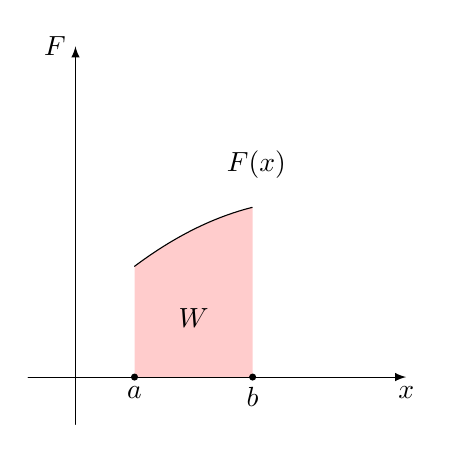
\begin{tikzpicture}
    [line cap=round,line join=round,x=2cm,y=2cm, scale=1.5, decoration={brace,amplitude=2pt}]
%main layer
%creating the ticks and xy-axis nodes
%some function
\fill[fill=red!20] (0.25,0) -- plot [domain=0.25:.75] (\x,{-\x^2/2+\x+0.25}) -- plot [domain=0.75: 0.25] (\x,0) -- cycle;

 \draw[smooth,samples=200,domain=0.25:0.75]
                                 plot(\x,{-\x^2/2+\x+0.25});
 

    \fill[black] (0.25,0) circle (0.3mm) node [anchor=north ,scale=1] {$ a$};
     \fill[black] (0.75,0) circle (0.3mm) node [anchor=north ,scale=1] {$b$};
      %  \fill[black] (0,0.25) circle (0.3mm) node [anchor=south east,scale=1] {\scriptsize$ v(0)$};

  \draw[-latex,color=black,thin] (-0.2,0) -- (1.4,0) node [anchor=north ,scale=1] {$x$};
   \draw[-latex,color=black,thin] (0,-0.2) -- (0,1.4)node [anchor=east ,scale=1] {$F$};
    \draw (0.6,0.8) node [anchor=south west ,scale=1] {$F(x)$};
        \draw (0.5,0.25) node [anchor=center ,scale=1] {$W$};
        
 \end{tikzpicture}
  \caption{Work is the area under the curve in a force versus position graph.}
  \label{fig:marginfig}
\end{marginfigure}


\newpage

\subsubsection{Case: Constant Force}
\newthought{In the case of constant force}, the work is graphically represented by a rectangular area.  Consider the constant force of gravity on a mass.  The work done by gravity is the product of the weight and the displacement.  With downward motion gravity does positive work.  In upward motion, gravity does negative work.
\begin{marginfigure}[-50pt]%
  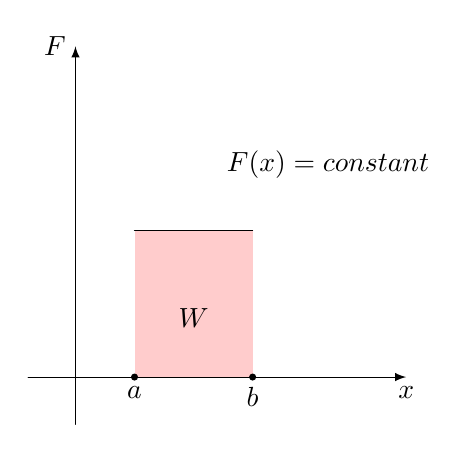
\begin{tikzpicture}
    [line cap=round,line join=round,x=2cm,y=2cm, scale=1.5, decoration={brace,amplitude=2pt}]
%main layer
%creating the ticks and xy-axis nodes
%some function
\fill[fill=red!20] (0.25,0) --(0.25, 0.62) -- (0.75, 0.62) -- (0.75,0.0) -- cycle;

 \draw (0.25, 0.62) -- (0.75, 0.62) ;
 

    \fill[black] (0.25,0) circle (0.3mm) node [anchor=north ,scale=1] {$ a$};
     \fill[black] (0.75,0) circle (0.3mm) node [anchor=north ,scale=1] {$b$};
      %  \fill[black] (0,0.25) circle (0.3mm) node [anchor=south east,scale=1] {\scriptsize$ v(0)$};

  \draw[-latex,color=black,thin] (-0.2,0) -- (1.4,0) node [anchor=north ,scale=1] {$x$};
   \draw[-latex,color=black,thin] (0,-0.2) -- (0,1.4)node [anchor=east ,scale=1] {$F$};
    \draw (0.6,0.8) node [anchor=south west ,scale=1] {$F(x)=\text{constant}$};
        \draw (0.5,0.25) node [anchor=center ,scale=1] {$W$};
        
 \end{tikzpicture}
  \caption{For a constant force, work is simply $F\cdot d$.}
  \label{fig:marginfig}
\end{marginfigure}

$$W=\text{Area}(F(x))$$
$$W=F(b-a)=F\Delta x$$

\vspace{1cm}

\subsubsection{Case: Linear Force}
\newthought{In the case of a force that is linearly proportional} to position, the work is graphically represented by the familiar region shown in Figure \ref{fig:linearwork}.  This area bay be represented mathematically as the difference between two triangular regions.

\begin{marginfigure}[0pt]%
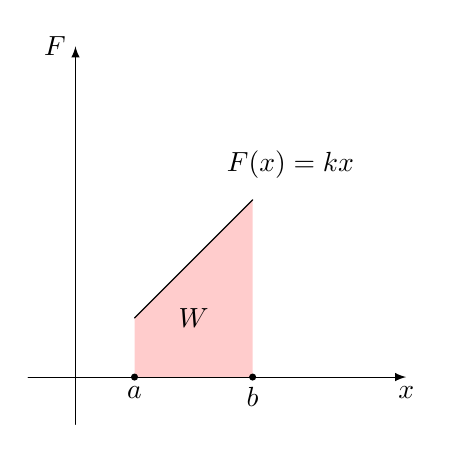
\begin{tikzpicture}
    [line cap=round,line join=round,x=2cm,y=2cm, scale=1.5, decoration={brace,amplitude=2pt}]
%main layer
%creating the ticks and xy-axis nodes
%some function
\fill[fill=red!20] (0.25,0) --(0.25, 0.25) -- (0.75, 0.75) -- (0.75,0.0) -- cycle;

 \draw (0.25, 0.25) -- (0.75, 0.75) ;
 

    \fill[black] (0.25,0) circle (0.3mm) node [anchor=north ,scale=1] {$ a$};
     \fill[black] (0.75,0) circle (0.3mm) node [anchor=north ,scale=1] {$b$};
      %  \fill[black] (0,0.25) circle (0.3mm) node [anchor=south east,scale=1] {\scriptsize$ v(0)$};

  \draw[-latex,color=black,thin] (-0.2,0) -- (1.4,0) node [anchor=north ,scale=1] {$x$};
   \draw[-latex,color=black,thin] (0,-0.2) -- (0,1.4)node [anchor=east ,scale=1] {$F$};
    \draw (0.6,0.8) node [anchor=south west ,scale=1] {$F(x)=kx$};
        \draw (0.5,0.25) node [anchor=center ,scale=1] {$W$};
        
 \end{tikzpicture}
  \caption{For a linear force, work is simply $\braket{F}\cdot d$.}
  \label{fig:linearwork}
\end{marginfigure}

$$W=\text{Area}(F(x))$$
$$W=\frac{kb^2}{2}-\frac{ka^2}{2}$$
$$W=\frac{k}{2}\left( b^2-a^2\right)=\frac{k}{2}\ \Delta( x^2)$$


 \subsection{2-D \& 3-D}

 \marginnote[0pt]{In higher dimensions, work is calculated as the dot product of the force and displacement vector.  For an arbitrary path sum the work over each section of the path.
 $$W=\sum_i \overrightarrow{F} \cdot \Delta{\overrightarrow{r}}_i$$}

The dot product is used to calculate work.  One interpretation is the product of displacement and force in the direction of displacement. 

\vspace{1cm}

 $$W=\overrightarrow{F}\cdot \Delta \overrightarrow{r}=F_{||} \  \Delta \overrightarrow{r}=F\cos\theta \  \Delta\overrightarrow{r}$$

\vspace{1cm}

$$
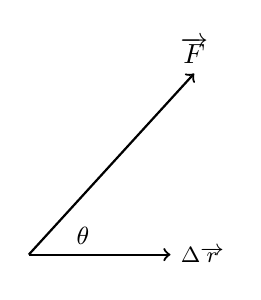
\begin{tikzpicture}[scale=1]
\draw [thick,->] (0,0) -- (2.1,2.3) node[anchor=south,color=black]{$\overrightarrow{F}$};
\draw [thick,->] (0,0) -- (1.8,0) node[midway, anchor=south east,color=black]{\small $\theta$} node[anchor=west,color=black]{\footnotesize$\Delta\overrightarrow{r}$};
\end{tikzpicture}
$$

\begin{marginfigure}[-80pt]%
\begin{tikzpicture}[scale=1.5]
\draw (2,0) node [anchor=north,scale=1] {$x $};
\draw (0,2) node [anchor=east,scale=1] {$y $};
\draw[->] (0,0) -- (2,0); 
\draw[->] (0,0) -- (0,2);
\fill[black] (0.45cm,1.05cm) circle (0.3mm);
\fill[black] (1.05cm,0.45cm) circle (0.3mm);
\draw (1,1) node [anchor=south west,scale=1] {$\{\Delta\overrightarrow{r}\}$};
\draw (0.5,1) node [anchor=south,scale=1] {$\ \ a$};
\draw (1,0.5) node [anchor=west,scale=1] {$\ b$};
\draw (0.5cm,1cm) [->,line width=0.2ex]  .. controls (0.6,0.6) and (0.8,0.8) ..   (1cm,0.5cm); 
\end{tikzpicture}
  \caption{Accumulation of work over a path.}
  \label{fig:linearwork}
\end{marginfigure}



\subsection{Unit}
\begin{marginfigure}%
  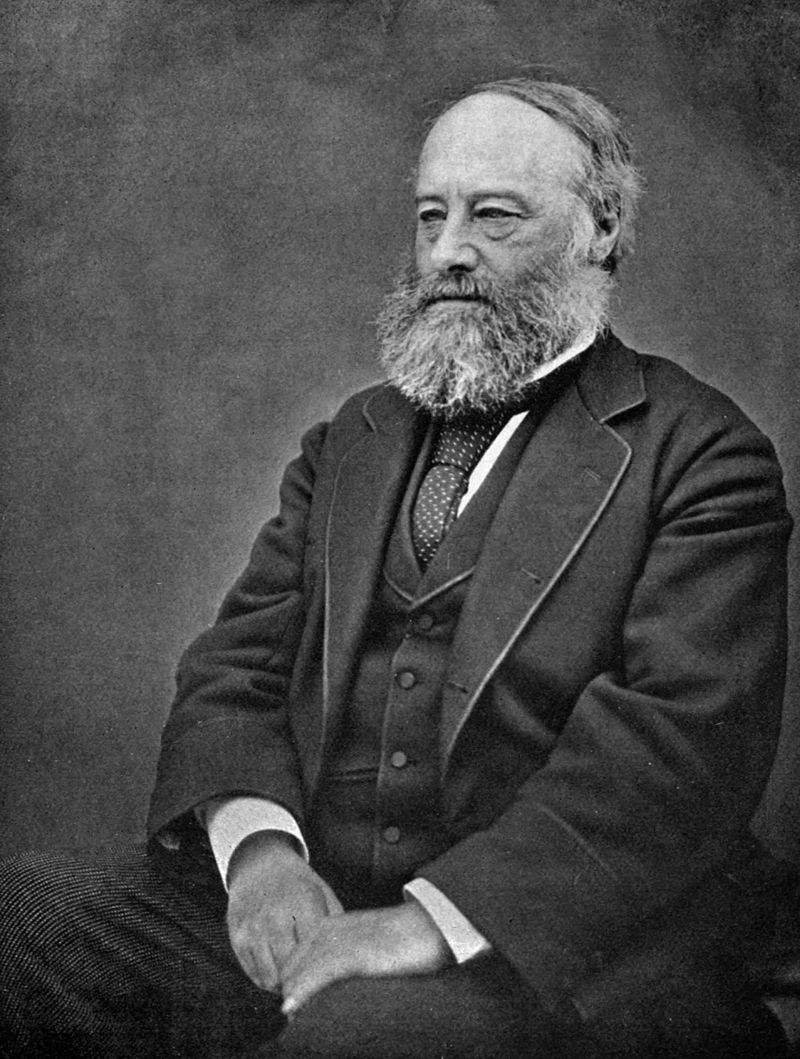
\includegraphics[width=\linewidth]{joule.jpg}
  \caption{James Joule rocked a three-piece suit.}
  \label{fig:marginfig}
\end{marginfigure}
\newthought{The Joule}, symbol J, is a derived unit of work and energy in the International System of Units.  It is equal to the work done to an object when a force of one newton acts on that object in the direction of its motion through a distance of one meter.  It is named after the English physicist James Prescott Joule (1818-1889).
$$\text{Joule}=\text{Newton}\cdot \text{meter}$$

\vspace{1cm}

\section{Power}
Power is the rate of doing work. It is equivalent to an amount of energy consumed per unit time. 
\begin{marginfigure}[0pt]%
  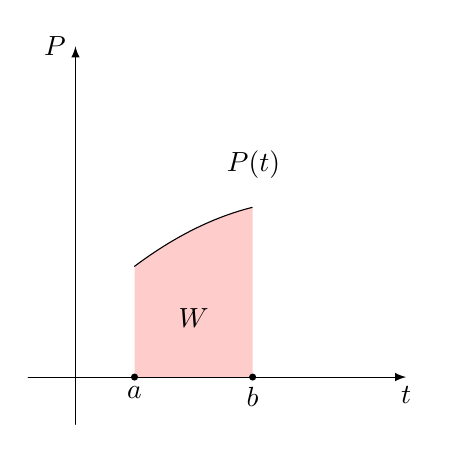
\begin{tikzpicture}
    [line cap=round,line join=round,x=2cm,y=2cm, scale=1.5, decoration={brace,amplitude=2pt}]
%main layer
%creating the ticks and xy-axis nodes
%some function
\fill[fill=red!20] (0.25,0) -- plot [domain=0.25:.75] (\x,{-\x^2/2+\x+0.25}) -- plot [domain=0.75: 0.25] (\x,0) -- cycle;

 \draw[smooth,samples=200,domain=0.25:0.75]
                                 plot(\x,{-\x^2/2+\x+0.25});
 

    \fill[black] (0.25,0) circle (0.3mm) node [anchor=north ,scale=1] {$ a$};
     \fill[black] (0.75,0) circle (0.3mm) node [anchor=north ,scale=1] {$b$};
      %  \fill[black] (0,0.25) circle (0.3mm) node [anchor=south east,scale=1] {\scriptsize$ v(0)$};

  \draw[-latex,color=black,thin] (-0.2,0) -- (1.4,0) node [anchor=north ,scale=1] {$t$};
   \draw[-latex,color=black,thin] (0,-0.2) -- (0,1.4)node [anchor=east ,scale=1] {$P$};
    \draw (0.6,0.8) node [anchor=south west ,scale=1] {$P(t)$};
        \draw (0.5,0.25) node [anchor=center ,scale=1] {$W$};
        
 \end{tikzpicture}
  \caption{Work is the area under the curve in a force versus position graph.}
  \label{fig:marginfig}
\end{marginfigure}

$$P=\frac{W}{\Delta t}$$
$$W=\text{Area}(P(t))$$
$$P=\frac{W}{\Delta t}=\frac{\overrightarrow{F}\cdot \Delta \overrightarrow{r}}{\Delta t}$$
$$P=\overrightarrow{F}\cdot  \overrightarrow{v}$$

\subsection{Unit}
\marginnote[5pt]{James Watt (1736-1819) was a Scottish inventor and mechanical engineer whose Watt steam engine was fundamental to the Industrial Revolution.}
In the SI system, the unit of power is the joule per second (J/s), known as the watt in honor of James Watt, the eighteenth-century developer of the steam engine.
$$\text{Watt}=\frac{\text{Joule}}{\text{second}}$$



\section{Kinetic Energy}
\begin{marginfigure}[20pt]%
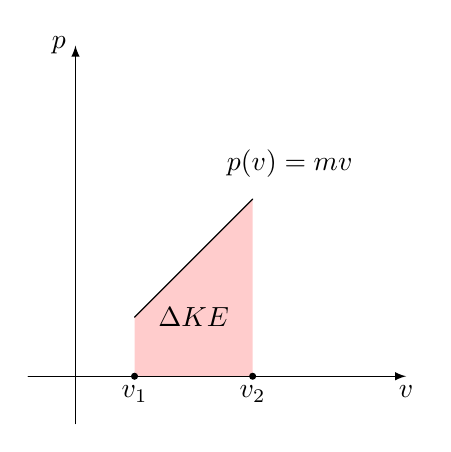
\begin{tikzpicture}
    [line cap=round,line join=round,x=2cm,y=2cm, scale=1.5, decoration={brace,amplitude=2pt}]
%main layer
%creating the ticks and xy-axis nodes
%some function
\fill[fill=red!20] (0.25,0) --(0.25, 0.25) -- (0.75, 0.75) -- (0.75,0.0) -- cycle;

 \draw (0.25, 0.25) -- (0.75, 0.75) ;
 

    \fill[black] (0.25,0) circle (0.3mm) node [anchor=north ,scale=1] {$ v_1$};
     \fill[black] (0.75,0) circle (0.3mm) node [anchor=north ,scale=1] {$v_2$};
      %  \fill[black] (0,0.25) circle (0.3mm) node [anchor=south east,scale=1] {\scriptsize$ v(0)$};

  \draw[-latex,color=black,thin] (-0.2,0) -- (1.4,0) node [anchor=north ,scale=1] {$v$};
   \draw[-latex,color=black,thin] (0,-0.2) -- (0,1.4)node [anchor=east ,scale=1] {$p$};
    \draw (0.6,0.8) node [anchor=south west ,scale=1] {$p(v)=mv$};
        \draw (0.5,0.25) node [anchor=center ,scale=1] {$\Delta KE$};
        
 \end{tikzpicture}
  \caption{Kinetic energy expressed as the area under p(v).}
  \label{fig:marginfig}
\end{marginfigure}

\newthought{The kinetic energy} of an object is the energy that it possesses due to its motion.  It is defined as the work needed to accelerate a body of a given mass from rest to its stated velocity. 



$$KE=\frac{pv}{2}=\frac{mv^2}{2}=\frac{p^2}{2m}$$
$$\Delta KE = KE_2-KE_1=\frac{mv_2^2}{2}-\frac{mv_1^2}{2}$$


\section{Work-Energy Theorem}
$$W_{net}=\Delta KE$$
The total work on a free rigid body is equal to the change in kinetic energy of that body.

\section{Path Independence and Conservative Forces}

\marginnote[0pt]{
\begin{itemize}
  \item Multiple Paths $\{\Delta \overrightarrow{r}\}_j$
  \item Each Path Has Work $W_j$ 
  \end{itemize}}

\begin{marginfigure}[0pt]
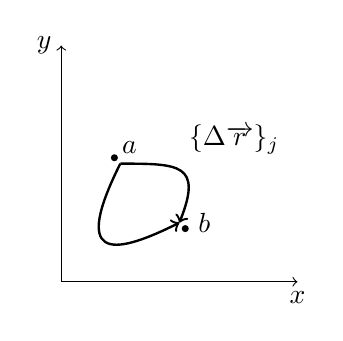
\begin{tikzpicture}[scale=1.5]
\draw (2,0) node [anchor=north,scale=1] {$x $};
\draw (0,2) node [anchor=east,scale=1] {$y $};
\draw[->] (0,0) -- (2,0); 
\draw[->] (0,0) -- (0,2);
\fill[black] (0.45cm,1.05cm) circle (0.3mm);
\fill[black] (1.05cm,0.45cm) circle (0.3mm);
\draw (1,1) node [anchor=south west,scale=1] {$\{\Delta\overrightarrow{r}\}_j$};
\draw (0.5,1) node [anchor=south,scale=1] {$\ \ a$};
\draw (1,0.5) node [anchor=west,scale=1] {$\ b$};
\draw (0.5cm,1cm) [->,line width=0.2ex]  .. controls (0.1,0.2) and (0.4,0.2) ..   (1cm,0.5cm); 
\draw (0.5cm,1cm) [->,line width=0.2ex]  .. controls (1,1) and (1.2,1) ..   (1cm,0.5cm); 
\end{tikzpicture}
 \caption{If the work from any possible path is identical then the underlying force is conservative.}
  \label{fig:marginfig}
\end{marginfigure}

\newthought{A conservative force is} a force with the property that the work done in moving a particle between two points is independent of the taken path.  Equivalently, if a particle travels in a closed loop, the net work done (the sum of the force acting along the path multiplied by the distance travelled) by a conservative force is zero.\\

A conservative force is dependent only on the position of the object. If a force is conservative, it is possible to assign a numerical value for the potential at any point. When an object moves from one location to another, the force changes the potential energy of the object by an amount that does not depend on the path taken. If the force is not conservative, then defining a scalar potential is not possible, because taking different paths would lead to conflicting potential differences between the start and end points.

Gravity is an example of a conservative force, while friction is an example of a non-conservative force.


\section{Potential Energy}
$$W_{cons}=-\Delta PE$$
\begin{marginfigure}[60pt]%
  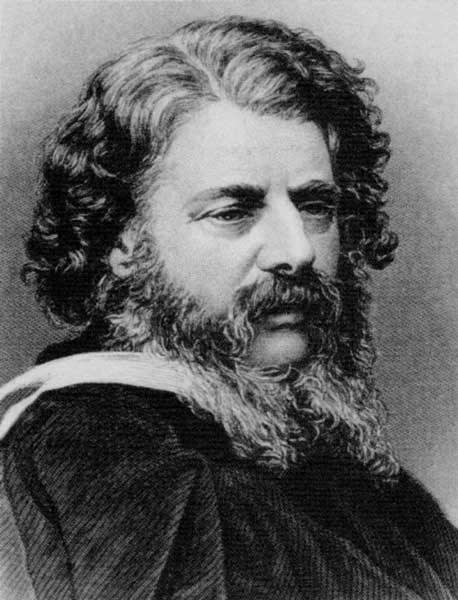
\includegraphics[width=\linewidth]{WilliamRankine.jpg}
  \caption{William Racine had boss facial hair.}
  \label{fig:marginfig}
\end{marginfigure}

\newthought{Potential energy} is the energy that an object has due to its position in a force field or that a system has due to the configuration of its parts.  Common types include the gravitational potential energy of an object that depends on its vertical position and mass, the elastic potential energy of an extended spring, and the electric potential energy of a charge in an electric field. The SI unit for energy is the Joule.

The term potential energy was introduced by the 19th century Scottish engineer and physicist William Rankine, although it has links to Greek philosopher Aristotle's concept of potentiality.  Work done by a conservative force is associated with a change in potential energy.  Potential energy is undefined up to a constant and therefore not a wholly tangible quantity.  The change in potential energy is a tangible quantity.



\section{Total Mechanical Energy}
\begin{marginfigure}[10pt]%
  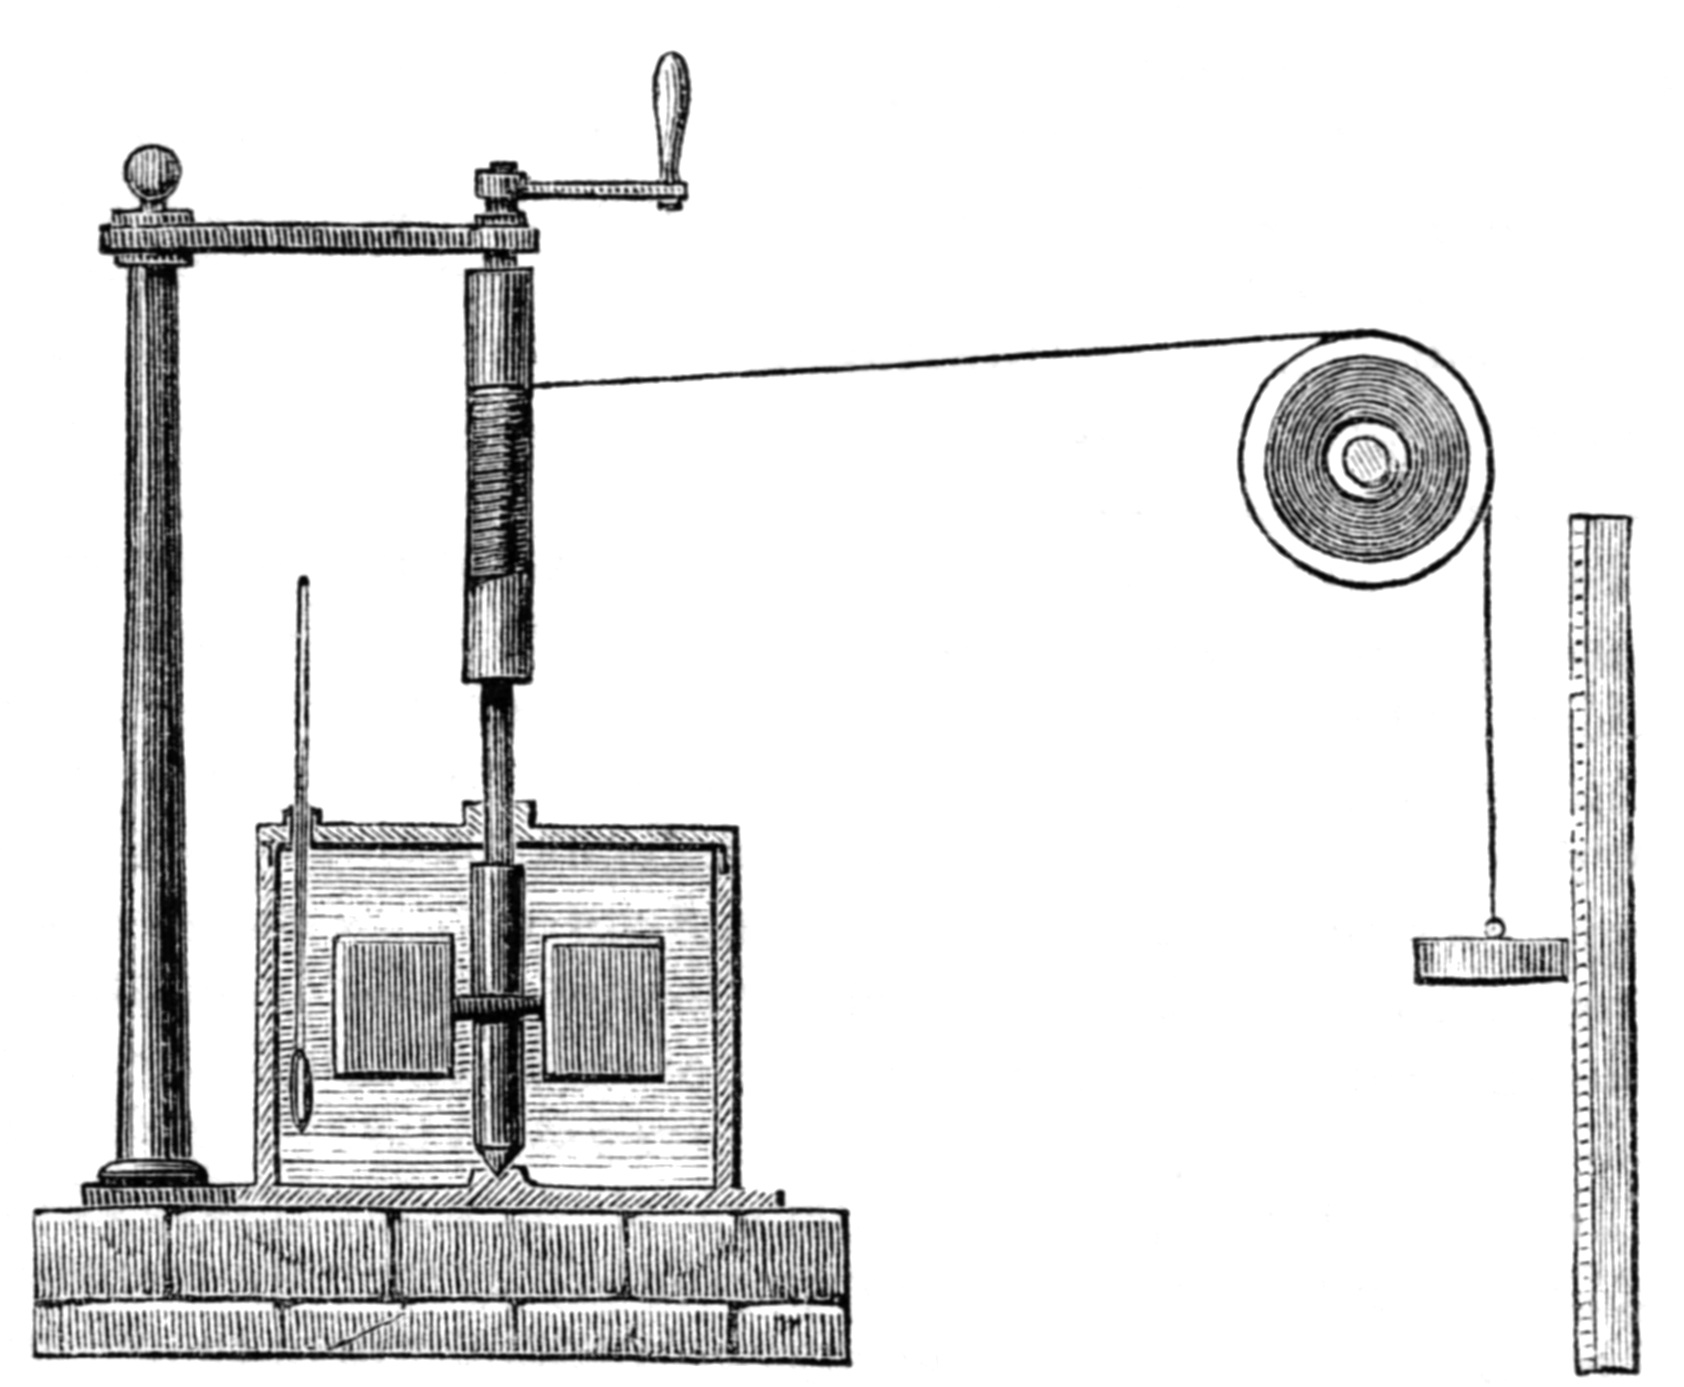
\includegraphics[width=\linewidth]{joule_ap.jpg}
  \caption{Joule's apparatus for measuring the mechanical equivalent of heat.}
  \label{fig:marginfig}
\end{marginfigure}
\newthought{Mechanical energy} is the sum of potential energy and kinetic energy.  The principle of conservation of mechanical energy states that in an isolated system that is only subject to conservative forces the mechanical energy is constant.  In all real systems, however, non-conservative forces, like frictional forces, will be present, but often they are of negligible values and the mechanical energy's being constant can therefore be a useful approximation. In elastic collisions, the mechanical energy is conserved but in inelastic collisions, some mechanical energy is converted into heat. 
$$E=KE+PE$$
$$W_{net}=W_{cons}+W_{non-cons}=\Delta KE$$
$$W_{non-cons}=\Delta{KE}+\Delta{PE}=\Delta(KE+PE)=\Delta{E}$$



\section{Gravitational Work and Potential Energy}
\marginnote[0pt]{Near the surface of the earth the force of gravity on a mass is a relatively constant weight, $mg$.  The potential energy associated with this constant force is the product of weight and displacement.  Note that the physicist chooses where the zero of potential energy is located. }
$$\overrightarrow{F}_g=-mg\hat{y}$$
$$W_g=-mg\ \Delta y$$
$$\Delta PE=-W_g=mg\ \Delta y$$
$$PE=mgy+\cancel{C}=mgy$$

\section{Spring Work and Potential Energy}
\marginnote[0pt]{For an ideal spring the resting force is Hookean.  In this case the potential energy is associated with the area of a triangle, 1/2 base $\times$ height.  The position of zero potential energy is typically taken as the equilibrium position.}
$$\overrightarrow{F}_k=-kx\hat{x}$$
$$W_k=-\frac{k(\Delta x)^2}{2}$$
$$\Delta PE=-W_k=\frac{k(\Delta x)^2}{2}$$
$$PE=\frac{kx^2}{2}+\cancel{C}=\frac{kx^2}{2}$$

\section{Universal Gravitational Work and Potential Energy}
\marginnote[0pt]{The potential energy associated with Newton's universal law of gravitation may seem strange at first glance.  It is negative, which might be confusing.  Verify the PE increases as a mass is moved father from the center of the earth.  Also note the position of zero potential energy is taken to be at infinity.}
$$\overrightarrow{F}_{g}=-\frac{Gm_1m_2}{r^2}\hat{r}$$
$$\Delta PE=-W_g=-\frac{Gm_1m_2}{r}$$
$$PE=-\frac{Gm_1m_2}{r}+\cancel{C}=-\frac{Gm_1m_2}{r}$$
\section{Frictional Work}
\marginnote[0pt]{Friction does not have a potential energy associated with it since it is a non-conservative force.  It is possible however to calculate the work done by friction.  The work done by friction ends up as heat energy.}
$$\overrightarrow{F}_{f}=-\mu_kF_n\hat{v}$$
$$W_f=\overrightarrow{F}_f\cdot \Delta \overrightarrow{r}$$
$$W_f=-\mu_k F_n\ \Delta x$$

Friction is a non-conservative force.

\section{Positive Work / Negative Work / No Work}
\begin{itemize}
  \item Positive Work- (Increases KE/speed) 
  \item Negative Work- (Decreases KE/speed)
  \item No Work- (KE/speed constant)
  \end{itemize}

\marginnote{
  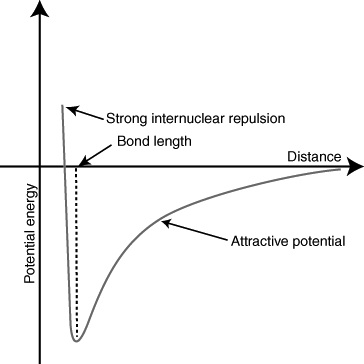
\includegraphics[width=\linewidth ]{peplot.jpg}}
  
  
  \section{Energy Diagrams}
  \begin{itemize}
  \item Potential Energy Wells
  \item  $E$, $PE(x)$, $KE(x)$
  \item Turning Points $KE(x_{turn})=0$
  \item Escape Energy and Escape Velocity
  \end{itemize}
